\documentclass[%
aps,
onecolumn,
11pt,
tightenlines,
nofootinbib,
superscriptaddress,
floatfix,
prd,
]{revtex4-2}

% ******************************************************
% ******************** BEGIN HEADER ********************
% ******************************************************

%%%%%%%%%%%%%%%%%%%%%%%%%%%%%%%%%%%%%%%%%%%%%%%%%%%%%%%%
%%%%%%%%%%%%%%%%%%%%%%%%%%%%%%%%%%%%%%%%%%%%%%%%%%%%%%%%
%%%PACKAGES
\usepackage{siunitx}
\usepackage{physics}
\usepackage{braket}

\usepackage{algorithm, algcompatible}
\usepackage{amsmath}	% AMS Math Package
\usepackage{amsthm}		% Theorem Formatting
\usepackage{amssymb}	% Math symbols such as \mathbb
\usepackage{anyfontsize}
\usepackage{booktabs}

\usepackage{mathrsfs, mathtools}

\usepackage{letltxmacro} % closed roots
\usepackage{caption}
\captionsetup{justification=centering}
\usepackage{color}
%\usepackage{verbatim}
\usepackage{bm}
%\usepackage{float}

\usepackage{tgpagella}

\usepackage{graphicx}
%\usepackage{xcolor}

\usepackage{fancyhdr}
\usepackage{float}

\usepackage{lastpage}

\usepackage{titlesec}

\usepackage{rotating}
\usepackage{setspace}

\usepackage[printonlyused]{acronym}
\usepackage{aas_macros}

%\usepackage{multirow}
\usepackage{datetime}

\usepackage{lettrine}

\usepackage{multirow}
\usepackage{parskip}
\usepackage{subcaption}


\usepackage[colorlinks=true
,urlcolor=DARKBLUE
,anchorcolor=DARKBLUE
,citecolor=DARKBLUE
,filecolor=DARKBLUE
,linkcolor=DARKBLUE
,menucolor=DARKBLUE
%,pagecolor=DARKBLUE
%,linktocpage=true
%,pdfproducer=medialab
%,pdfa=true
]{hyperref}
%\hypersetup{
 %   colorlinks,
  %  linkcolor={red!50!black},
   % citecolor={blue!50!black},
    %urlcolor={blue!80!black}
%}

%\usepackage[square, sort, comma, numbers]{natbib}

\def\bibsection{} %remove black horizontal line before references

\titleformat{\section}
       {\centering\normalfont\fontsize{14}{17}\bfseries}{\thesection}{1em}{}

\numberwithin{equation}{section}

\renewcommand{\figurename}{{\bf Figure}}
\renewcommand{\tablename}{{\bf Table}}

\makeatletter 
    \renewcommand{\thefigure}{{\bf\@arabic\c@figure}}
\makeatother

%\makeatletter
%\renewenvironment{abstract}{%
%    \begin{center}%

%       {\bfseries \Large\abstractname\vspace{\z@}}%  %% <- here I've added \Large
%     \end{center}%
%    \quotation}
%\makeatother

%\acrodef{CDM}[CDM]{cold dark matter}
%\acrodef{CDM}[CDM]{cold dark matter}
%\acrodef{CMB}[CMB]{cosmic microwave background}
%\acrodef{EoM}[EoM]{equation of motion}
%    \acrodefplural{EoM}[EoMs]{equations of motion}
%\acrodef{LSS}[LSS]{large scale structure}
%\acrodef{NG}[NG]{non-Gaussianity}
%    \acrodefplural{NG}[NGs]{non-Gaussianities}
%\acrodef{PBH}[PBH]{primordial black hole}
%    \acrodefplural{PBH}[PBHs]{primordial black holes}
%\acrodef{SR}[SR]{slow-roll}
%\acrodef{WIMP}[WIMP]{weakly-interacting massive particle}
%    \acrodefplural{WIMP}[WIMPs]{weakly-interacting massive particles}
    
%\acrodef{PBH}{primordial black hole}
%\acrodef{SR}{slow-roll}
%\acrodef{NG}{non-Gaussianity}
%\acrodef{EoM}{equation of motion}
%\acrodef{CMB}{cosmic microwave background}
%\acrodef{LSS}{large scale structure}

%\bibliographystyle{apsrev4-2}

\usepackage{tcolorbox}
%\definecolor{block-gray}{gray}{0.92}
%\newtcolorbox{newquote}{colback=block-gray, grow to right by=-5mm, grow to left by=-5mm, boxrule=1pt, boxsep=5pt, breakable
%}


\fancyhf{}
\chead[odd]{
Versuchsprotokoll - 16: $\gamma - \gamma-$Koinzidenzen
\vphantom{$_{_{_{}}}$}}

\cfoot{ \fancyplain{}{-- \thepage}/{\pageref{LastPage}} --}



%%%%%%%%%%%%%%%%%%%%%%%%%%%%%%%%%%%%%%%%%%%%%%%%%%%%%%%%
%%%%%%%%%%%%%%%%%%%%%%%%%%%%%%%%%%%%%%%%%%%%%%%%%%%%%%%%
%%%COLOURS
%existing: black, white, blue, red, green, yellow
\definecolor{grey}{rgb}{0.4,0.4,0.4}
\definecolor{dullmagenta}{rgb}{0.4,0,0.4}
\definecolor{darkblue}{rgb}{0,0,0.4}
\definecolor{midblue}{rgb}{0,0,0.7}
\definecolor{midred}{rgb}{0.5,0,0}
\definecolor{orange}{rgb}{1,0.5,0}
\definecolor{lightbrown}{rgb}{0.75,0.5,0.25}
\definecolor{tan}{cmyk}{0.14,0.42,0.56,0}
\definecolor{djunglegreen}{cmyk}{0.99,0,0.52,0}
\definecolor{lightgreen}{rgb}{0,1,0}
\definecolor{olivegreen}{cmyk}{0.64,0,0.95,0.40}
\definecolor{midgreen}{rgb}{0.0,0.675,0.0}
\definecolor{darkgreen}{rgb}{0,0.5,0}
\definecolor{pink}{rgb}{1,0.078,0.57}

\definecolor{MONZA}{HTML}{CF000F}
\definecolor{DARKBLUE}{HTML}{00008b}
\definecolor{DARKMAGENTA}{HTML}{8b008b}


%%%%%%%%%%%%%%%%%%%%%%%%%%%%%%%%%%%%%%%%%%%%%%%%%%%%%%%%
%%%%%%%%%%%%%%%%%%%%%%%%%%%%%%%%%%%%%%%%%%%%%%%%%%%%%%%%
%%%NORMS
\newcommand{\normsingle}[1]{\left|{#1}\right|}
\newcommand{\normdouble}[1]{\left\|{#1}\right\|}
%\newcommand{\normtriple}[1]{\left\interleave{#1}\right\interleave} % requires ``stmaryrd'' package
%\newcommand{\norm}[1]{\normdouble{#1}}



%%%%%%%%%%%%%%%%%%%%%%%%%%%%%%%%%%%%%%%%%%%%%%%%%%%%%%%%
%%%%%%%%%%%%%%%%%%%%%%%%%%%%%%%%%%%%%%%%%%%%%%%%%%%%%%%%
%%%SHIFTS
\newcommand{\q}{\quad}
%\newcommand{\qq}{\qquad}
\newcommand{\qqq}{\qquad\quad}
\newcommand{\qqqq}{\qquad\qquad}
\newcommand{\vs}{\vspace}
\newcommand{\hs}{\hspace}
\renewcommand{\.}{\hspace{0.5mm}}



%%%%%%%%%%%%%%%%%%%%%%%%%%%%%%%%%%%%%%%%%%%%%%%%%%%%%%%%
%%%%%%%%%%%%%%%%%%%%%%%%%%%%%%%%%%%%%%%%%%%%%%%%%%%%%%%%
%%%CLOSED ROOTS
\makeatletter
\let\oldr@@t\r@@t
\def\r@@t#1#2{%
\setbox0=\hbox{$\oldr@@t#1{#2\,}$}\dimen0=\ht0
\advance\dimen0-0.2\ht0
\setbox2=\hbox{\vrule height\ht0 depth -\dimen0}%
{\box0\lower0.4pt\box2}}
\LetLtxMacro{\oldsqrt}{\sqrt}
\renewcommand*{\sqrt}[2][\ ]{\oldsqrt[#1]{#2}}
\makeatother



%%%%%%%%%%%%%%%%%%%%%%%%%%%%%%%%%%%%%%%%%%%%%%%%%%%%%%%%
%%%%%%%%%%%%%%%%%%%%%%%%%%%%%%%%%%%%%%%%%%%%%%%%%%%%%%%%
%%%ARROWS
\newcommand{\ra}{\ensuremath{\rightarrow}}
\newcommand{\la}{\ensuremath{\leftarrow}}
\newcommand{\Ra}{\ensuremath{\Rightarrow}}
\newcommand{\La}{\ensuremath{\Leftarrow}}
\newcommand{\lra}{\ensuremath{\leftrightarrow}}
\newcommand{\Lra}{\ensuremath{\Leftrightarrow}}
\newcommand{\Ral}{\ensuremath{\Longrightarrow}}
\newcommand{\Lal}{\ensuremath{\Longleftarrow}}
\newcommand{\Lral}{\ensuremath{\Longleftrightarrow}}
\newcommand{\lral}{\ensuremath{\ongleftrightarrow}}
\newcommand{\ral}{\ensuremath{\longrightarrow}}
\newcommand{\lal}{\ensuremath{\longleftarrow}}



%%%%%%%%%%%%%%%%%%%%%%%%%%%%%%%%%%%%%%%%%%%%%%%%%%%%%%%%
%%%%%%%%%%%%%%%%%%%%%%%%%%%%%%%%%%%%%%%%%%%%%%%%%%%%%%%%
%%%MATHEMATICS

%%%capital \mathrm
\newcommand{\Arm}{\ensuremath{\mathrm{A}}}
\newcommand{\Brm}{\ensuremath{\mathrm{B}}}
\newcommand{\Crm}{\ensuremath{\mathrm{C}}}
\newcommand{\Drm}{\ensuremath{\mathrm{D}}}
\newcommand{\Erm}{\ensuremath{\mathrm{E}}}
\newcommand{\Frm}{\ensuremath{\mathrm{F}}}
\newcommand{\Grm}{\ensuremath{\mathrm{G}}}
\newcommand{\Hrm}{\ensuremath{\mathrm{H}}}
\newcommand{\Irm}{\ensuremath{\mathrm{I}}}
\newcommand{\Jrm}{\ensuremath{\mathrm{J}}}
\newcommand{\Krm}{\ensuremath{\mathrm{K}}}
\newcommand{\Lrm}{\ensuremath{\mathrm{L}}}
\newcommand{\Mrm}{\ensuremath{\mathrm{M}}}
\newcommand{\Nrm}{\ensuremath{\mathrm{N}}}
\newcommand{\Orm}{\ensuremath{\mathrm{O}}}
\newcommand{\Prm}{\ensuremath{\mathrm{P}}}
\newcommand{\Qrm}{\ensuremath{\mathrm{Q}}}
\newcommand{\Rrm}{\ensuremath{\mathrm{R}}}
\newcommand{\Srm}{\ensuremath{\mathrm{S}}}
\newcommand{\Trm}{\ensuremath{\mathrm{T}}}
\newcommand{\Urm}{\ensuremath{\mathrm{U}}}
\newcommand{\Vrm}{\ensuremath{\mathrm{V}}}
\newcommand{\Wrm}{\ensuremath{\mathrm{W}}}
\newcommand{\Xrm}{\ensuremath{\mathrm{X}}}
\newcommand{\Yrm}{\ensuremath{\mathrm{Y}}}
\newcommand{\Zrm}{\ensuremath{\mathrm{Z}}}
%%%small \mathrm
\newcommand{\arm}{\ensuremath{\mathrm{a}}}
\newcommand{\brm}{\ensuremath{\mathrm{b}}}
\newcommand{\crm}{\ensuremath{\mathrm{c}}}
\newcommand{\drm}{\ensuremath{\mathrm{d}}}
\newcommand{\erm}{\ensuremath{\mathrm{e}}}
\newcommand{\frm}{\ensuremath{\mathrm{f}}}
\newcommand{\grm}{\ensuremath{\mathrm{g}}}
\newcommand{\hrm}{\ensuremath{\mathrm{h}}}
\newcommand{\irm}{\ensuremath{\mathrm{i}}}
\newcommand{\jrm}{\ensuremath{\mathrm{j}}}
\newcommand{\krm}{\ensuremath{\mathrm{k}}}
\newcommand{\lrm}{\ensuremath{\mathrm{l}}}
\newcommand{\mrm}{\ensuremath{\mathrm{m}}}
\newcommand{\nrm}{\ensuremath{\mathrm{n}}}
\newcommand{\orm}{\ensuremath{\mathrm{o}}}
\newcommand{\prm}{\ensuremath{\mathrm{p}}}
\newcommand{\qrm}{\ensuremath{\mathrm{q}}}
\newcommand{\rrm}{\ensuremath{\mathrm{r}}}
\newcommand{\srm}{\ensuremath{\mathrm{s}}}
\newcommand{\trm}{\ensuremath{\mathrm{t}}}
\newcommand{\urm}{\ensuremath{\mathrm{u}}}
\newcommand{\vrm}{\ensuremath{\mathrm{v}}}
\newcommand{\wrm}{\ensuremath{\mathrm{w}}}
\newcommand{\xrm}{\ensuremath{\mathrm{x}}}
\newcommand{\yrm}{\ensuremath{\mathrm{y}}}
\newcommand{\zrm}{\ensuremath{\mathrm{z}}}

%%%capital \mathcal
\newcommand{\Acal}{\ensuremath{\mathcal{A}}}
\newcommand{\Bcal}{\ensuremath{\mathcal{B}}}
\newcommand{\Ccal}{\ensuremath{\mathcal{C}}}
\newcommand{\Dcal}{\ensuremath{\mathcal{D}}}
\newcommand{\Ecal}{\ensuremath{\mathcal{E}}}
\newcommand{\Fcal}{\ensuremath{\mathcal{F}}}
\newcommand{\Gcal}{\ensuremath{\mathcal{G}}}
\newcommand{\Hcal}{\ensuremath{\mathcal{H}}}
\newcommand{\Ical}{\ensuremath{\mathcal{I}}}
\newcommand{\Jcal}{\ensuremath{\mathcal{J}}}
\newcommand{\Kcal}{\ensuremath{\mathcal{K}}}
\newcommand{\Lcal}{\ensuremath{\mathcal{L}}}
\newcommand{\Mcal}{\ensuremath{\mathcal{M}}}
\newcommand{\Ncal}{\ensuremath{\mathcal{N}}}
\newcommand{\Ocal}{\ensuremath{\mathcal{O}}}
\newcommand{\Pcal}{\ensuremath{\mathcal{P}}}
\newcommand{\Qcal}{\ensuremath{\mathcal{Q}}}
\newcommand{\Rcal}{\ensuremath{\mathcal{R}}}
\newcommand{\Scal}{\ensuremath{\mathcal{S}}}
\newcommand{\Tcal}{\ensuremath{\mathcal{T}}}
\newcommand{\Ucal}{\ensuremath{\mathcal{U}}}
\newcommand{\Vcal}{\ensuremath{\mathcal{V}}}
\newcommand{\Wcal}{\ensuremath{\mathcal{W}}}
\newcommand{\Xcal}{\ensuremath{\mathcal{X}}}
\newcommand{\Ycal}{\ensuremath{\mathcal{Y}}}
\newcommand{\Zcal}{\ensuremath{\mathcal{Z}}}

%%%capital \mathsf
\newcommand{\Asf}{\ensuremath{\mathsf{A}}}
\newcommand{\Bsf}{\ensuremath{\mathsf{B}}}
\newcommand{\Csf}{\ensuremath{\mathsf{C}}}
\newcommand{\Dsf}{\ensuremath{\mathsf{D}}}
\newcommand{\Esf}{\ensuremath{\mathsf{E}}}
\newcommand{\Fsf}{\ensuremath{\mathsf{F}}}
\newcommand{\Gsf}{\ensuremath{\mathsf{G}}}
\newcommand{\Hsf}{\ensuremath{\mathsf{H}}}
\newcommand{\Isf}{\ensuremath{\mathsf{I}}}
\newcommand{\Jsf}{\ensuremath{\mathsf{J}}}
\newcommand{\Ksf}{\ensuremath{\mathsf{K}}}
\newcommand{\Lsf}{\ensuremath{\mathsf{L}}}
\newcommand{\Msf}{\ensuremath{\mathsf{M}}}
\newcommand{\Nsf}{\ensuremath{\mathsf{N}}}
\newcommand{\Osf}{\ensuremath{\mathsf{O}}}
\newcommand{\Psf}{\ensuremath{\mathsf{P}}}
\newcommand{\Qsf}{\ensuremath{\mathsf{Q}}}
\newcommand{\Rsf}{\ensuremath{\mathsf{R}}}
\newcommand{\Ssf}{\ensuremath{\mathsf{S}}}
\newcommand{\Tsf}{\ensuremath{\mathsf{T}}}
\newcommand{\Usf}{\ensuremath{\mathsf{U}}}
\newcommand{\Vsf}{\ensuremath{\mathsf{V}}}
\newcommand{\Wsf}{\ensuremath{\mathsf{W}}}
\newcommand{\Xsf}{\ensuremath{\mathsf{X}}}
\newcommand{\Ysf}{\ensuremath{\mathsf{Y}}}
\newcommand{\Zsf}{\ensuremath{\mathsf{Z}}}
%%%small \mathcal
\newcommand{\asf}{\ensuremath{\mathsf{a}}}
\newcommand{\bsf}{\ensuremath{\mathsf{b}}}
\newcommand{\csf}{\ensuremath{\mathsf{c}}}
\newcommand{\dsf}{\ensuremath{\mathsf{d}}}
\newcommand{\esf}{\ensuremath{\mathsf{e}}}
\newcommand{\fsf}{\ensuremath{\mathsf{f}}}
\newcommand{\gsf}{\ensuremath{\mathsf{g}}}
\newcommand{\hsf}{\ensuremath{\mathsf{h}}}
\newcommand{\isf}{\ensuremath{\mathsf{i}}}
\newcommand{\jsf}{\ensuremath{\mathsf{j}}}
\newcommand{\ksf}{\ensuremath{\mathsf{k}}}
\newcommand{\lsf}{\ensuremath{\mathsf{l}}}
\newcommand{\msf}{\ensuremath{\mathsf{m}}}
\newcommand{\nsf}{\ensuremath{\mathsf{n}}}
\newcommand{\osf}{\ensuremath{\mathsf{o}}}
\newcommand{\psf}{\ensuremath{\mathsf{p}}}
\newcommand{\qsf}{\ensuremath{\mathsf{q}}}
\newcommand{\rsf}{\ensuremath{\mathsf{r}}}
\newcommand{\ssf}{\ensuremath{\mathsf{s}}}
\newcommand{\tsf}{\ensuremath{\mathsf{t}}}
\newcommand{\usf}{\ensuremath{\mathsf{u}}}
\newcommand{\vsf}{\ensuremath{\mathsf{v}}}
\newcommand{\wsf}{\ensuremath{\mathsf{w}}}
\newcommand{\xsf}{\ensuremath{\mathsf{x}}}
\newcommand{\ysf}{\ensuremath{\mathsf{y}}}
\newcommand{\zsf}{\ensuremath{\mathsf{z}}}

%%%capital \mathbb
\newcommand{\Abb}{\ensuremath{\mathbb{A}}}
\renewcommand{\Bbb}{\ensuremath{\mathbb{B}}}
\newcommand{\Cbb}{\ensuremath{\mathbb{C}}}
\newcommand{\Dbb}{\ensuremath{\mathbb{D}}}
\newcommand{\Ebb}{\ensuremath{\mathbb{E}}}
\newcommand{\Fbb}{\ensuremath{\mathbb{F}}}
\newcommand{\Gbb}{\ensuremath{\mathbb{G}}}
\newcommand{\Hbb}{\ensuremath{\mathbb{H}}}
\newcommand{\Ibb}{\ensuremath{\mathbb{I}}}
\newcommand{\Jbb}{\ensuremath{\mathbb{J}}}
\newcommand{\Kbb}{\ensuremath{\mathbb{K}}}
\newcommand{\Lbb}{\ensuremath{\mathbb{L}}}
\newcommand{\Mbb}{\ensuremath{\mathbb{M}}}
\newcommand{\Nbb}{\ensuremath{\mathbb{N}}}
\newcommand{\Obb}{\ensuremath{\mathbb{O}}}
\newcommand{\Pbb}{\ensuremath{\mathbb{P}}}
\newcommand{\Qbb}{\ensuremath{\mathbb{Q}}}
\newcommand{\Rbb}{\ensuremath{\mathbb{R}}}
\newcommand{\Sbb}{\ensuremath{\mathbb{S}}}
\newcommand{\Tbb}{\ensuremath{\mathbb{T}}}
\newcommand{\Ubb}{\ensuremath{\mathbb{U}}}
\newcommand{\Vbb}{\ensuremath{\mathbb{V}}}
\newcommand{\Wbb}{\ensuremath{\mathbb{W}}}
\newcommand{\Xbb}{\ensuremath{\mathbb{X}}}
\newcommand{\Ybb}{\ensuremath{\mathbb{Y}}}
\newcommand{\Zbb}{\ensuremath{\mathbb{Z}}}
%%%small \mathbb
\newcommand{\abb}{\ensuremath{\mathbb{a}}}
\newcommand{\bbb}{\ensuremath{\mathbb{b}}}
\newcommand{\cbb}{\ensuremath{\mathbb{c}}}
\newcommand{\dbb}{\ensuremath{\mathbb{d}}}
\newcommand{\ebb}{\ensuremath{\mathbb{e}}}
\newcommand{\fbb}{\ensuremath{\mathbb{f}}}
\newcommand{\gbb}{\ensuremath{\mathbb{g}}}
\newcommand{\hbb}{\ensuremath{\mathbb{h}}}
\newcommand{\ibb}{\ensuremath{\mathbb{i}}}
\newcommand{\jbb}{\ensuremath{\mathbb{j}}}
\newcommand{\kbb}{\ensuremath{\mathbb{k}}}
\newcommand{\lbb}{\ensuremath{\mathbb{l}}}
\newcommand{\mbb}{\ensuremath{\mathbb{m}}}
\newcommand{\nbb}{\ensuremath{\mathbb{n}}}
\newcommand{\obb}{\ensuremath{\mathbb{o}}}
\newcommand{\pbb}{\ensuremath{\mathbb{p}}}
\newcommand{\qbb}{\ensuremath{\mathbb{q}}}
\newcommand{\rbb}{\ensuremath{\mathbb{r}}}
\newcommand{\sbb}{\ensuremath{\mathbb{s}}}
\newcommand{\tbb}{\ensuremath{\mathbb{t}}}
\newcommand{\ubb}{\ensuremath{\mathbb{u}}}
\newcommand{\vbb}{\ensuremath{\mathbb{v}}}
\newcommand{\wbb}{\ensuremath{\mathbb{w}}}
\newcommand{\xbb}{\ensuremath{\mathbb{x}}}
\newcommand{\ybb}{\ensuremath{\mathbb{y}}}
\newcommand{\zbb}{\ensuremath{\mathbb{z}}}

%%%capital \mathbbm
\newcommand{\Abbm}{\ensuremath{\mathbbm{A}}}
\newcommand{\Bbbm}{\ensuremath{\mathbbm{B}}}
\newcommand{\Cbbm}{\ensuremath{\mathbbm{C}}}
\newcommand{\Dbbm}{\ensuremath{\mathbbm{D}}}
\newcommand{\Ebbm}{\ensuremath{\mathbbm{E}}}
\newcommand{\Fbbm}{\ensuremath{\mathbbm{F}}}
\newcommand{\Gbbm}{\ensuremath{\mathbbm{G}}}
\newcommand{\Hbbm}{\ensuremath{\mathbbm{H}}}
\newcommand{\Ibbm}{\ensuremath{\mathbbm{I}}}
\newcommand{\Jbbm}{\ensuremath{\mathbbm{J}}}
\newcommand{\Kbbm}{\ensuremath{\mathbbm{K}}}
\newcommand{\Lbbm}{\ensuremath{\mathbbm{L}}}
\newcommand{\Mbbm}{\ensuremath{\mathbbm{M}}}
\newcommand{\Nbbm}{\ensuremath{\mathbbm{N}}}
\newcommand{\Obbm}{\ensuremath{\mathbbm{O}}}
\newcommand{\Pbbm}{\ensuremath{\mathbbm{P}}}
\newcommand{\Qbbm}{\ensuremath{\mathbbm{Q}}}
\newcommand{\Rbbm}{\ensuremath{\mathbbm{R}}}
\newcommand{\Sbbm}{\ensuremath{\mathbbm{S}}}
\newcommand{\Tbbm}{\ensuremath{\mathbbm{T}}}
\newcommand{\Ubbm}{\ensuremath{\mathbbm{U}}}
\newcommand{\Vbbm}{\ensuremath{\mathbbm{V}}}
\newcommand{\Wbbm}{\ensuremath{\mathbbm{W}}}
\newcommand{\Xbbm}{\ensuremath{\mathbbm{X}}}
\newcommand{\Ybbm}{\ensuremath{\mathbbm{Y}}}
\newcommand{\Zbbm}{\ensuremath{\mathbbm{Z}}}
%%%small \mathbbm
\newcommand{\abbm}{\ensuremath{\mathbbm{a}}}
\newcommand{\bbbm}{\ensuremath{\mathbbm{b}}}
\newcommand{\cbbm}{\ensuremath{\mathbbm{c}}}
\newcommand{\dbbm}{\ensuremath{\mathbbm{d}}}
\newcommand{\ebbm}{\ensuremath{\mathbbm{e}}}
\newcommand{\fbbm}{\ensuremath{\mathbbm{f}}}
\newcommand{\gbbm}{\ensuremath{\mathbbm{g}}}
\newcommand{\hbbm}{\ensuremath{\mathbbm{h}}}
\newcommand{\ibbm}{\ensuremath{\mathbbm{i}}}
\newcommand{\jbbm}{\ensuremath{\mathbbm{j}}}
\newcommand{\kbbm}{\ensuremath{\mathbbm{k}}}
\newcommand{\lbbm}{\ensuremath{\mathbbm{l}}}
\newcommand{\mbbm}{\ensuremath{\mathbbm{m}}}
\newcommand{\nbbm}{\ensuremath{\mathbbm{n}}}
\newcommand{\obbm}{\ensuremath{\mathbbm{o}}}
\newcommand{\pbbm}{\ensuremath{\mathbbm{p}}}
\newcommand{\qbbm}{\ensuremath{\mathbbm{q}}}
\newcommand{\rbbm}{\ensuremath{\mathbbm{r}}}
\newcommand{\sbbm}{\ensuremath{\mathbbm{s}}}
\newcommand{\tbbm}{\ensuremath{\mathbbm{t}}}
\newcommand{\ubbm}{\ensuremath{\mathbbm{u}}}
\newcommand{\vbbm}{\ensuremath{\mathbbm{v}}}
\newcommand{\wbbm}{\ensuremath{\mathbbm{w}}}
\newcommand{\xbbm}{\ensuremath{\mathbbm{x}}}
\newcommand{\ybbm}{\ensuremath{\mathbbm{y}}}
\newcommand{\zbbm}{\ensuremath{\mathbbm{z}}}
%%%numbers \mathbbm
\newcommand{\zerobbm}{\ensuremath{\mathbbm{0}}}
\newcommand{\onebbm}{\ensuremath{\mathbbm{1}}}
\newcommand{\twobbm}{\ensuremath{\mathbbm{2}}}
\newcommand{\fourbbm}{\ensuremath{\mathbbm{3}}}
\newcommand{\fifebbm}{\ensuremath{\mathbbm{3}}}
\newcommand{\sixbbm}{\ensuremath{\mathbbm{3}}}
\newcommand{\sevenbbm}{\ensuremath{\mathbbm{3}}}
\newcommand{\eightbbm}{\ensuremath{\mathbbm{3}}}
\newcommand{\ninebbm}{\ensuremath{\mathbbm{3}}}


%%%capital \mathbm
\newcommand{\Abm}{\ensuremath{\bm{A}}}
\newcommand{\Bbm}{\ensuremath{\bm{B}}}
\newcommand{\Cbm}{\ensuremath{\bm{C}}}
\newcommand{\Dbm}{\ensuremath{\bm{D}}}
\newcommand{\Ebm}{\ensuremath{\bm{E}}}
\newcommand{\Fbm}{\ensuremath{\bm{F}}}
\newcommand{\Gbm}{\ensuremath{\bm{G}}}
\newcommand{\Hbm}{\ensuremath{\bm{H}}}
\newcommand{\Ibm}{\ensuremath{\bm{I}}}
\newcommand{\Jbm}{\ensuremath{\bm{J}}}
\newcommand{\Kbm}{\ensuremath{\bm{K}}}
\newcommand{\Lbm}{\ensuremath{\bm{L}}}
\newcommand{\Mbm}{\ensuremath{\bm{M}}}
\newcommand{\Nbm}{\ensuremath{\bm{N}}}
\newcommand{\Obm}{\ensuremath{\bm{O}}}
\newcommand{\Pbm}{\ensuremath{\bm{P}}}
\newcommand{\Qbm}{\ensuremath{\bm{Q}}}
\newcommand{\Rbm}{\ensuremath{\bm{R}}}
\newcommand{\Sbm}{\ensuremath{\bm{S}}}
\newcommand{\Tbm}{\ensuremath{\bm{T}}}
\newcommand{\Ubm}{\ensuremath{\bm{U}}}
\newcommand{\Vbm}{\ensuremath{\bm{V}}}
\newcommand{\Wbm}{\ensuremath{\bm{W}}}
\newcommand{\Xbm}{\ensuremath{\bm{X}}}
\newcommand{\Ybm}{\ensuremath{\bm{Y}}}
\newcommand{\Zbm}{\ensuremath{\bm{Z}}}
%%%small \mathbm
\newcommand{\abm}{\ensuremath{\bm{a}}}
\newcommand{\bbm}{\ensuremath{\bm{b}}}
\newcommand{\cbm}{\ensuremath{\bm{c}}}
\newcommand{\dbm}{\ensuremath{\bm{d}}}
\newcommand{\ebm}{\ensuremath{\bm{e}}}
\newcommand{\fbm}{\ensuremath{\bm{f}}}
\newcommand{\gbm}{\ensuremath{\bm{g}}}
\newcommand{\hbm}{\ensuremath{\bm{h}}}
\newcommand{\ibm}{\ensuremath{\bm{i}}}
\newcommand{\jbm}{\ensuremath{\bm{j}}}
\newcommand{\kbm}{\ensuremath{\bm{k}}}
\newcommand{\lbm}{\ensuremath{\bm{l}}}
\newcommand{\mbm}{\ensuremath{\bm{m}}}
\newcommand{\nbm}{\ensuremath{\bm{n}}}
\newcommand{\obm}{\ensuremath{\bm{o}}}
\newcommand{\pbm}{\ensuremath{\bm{p}}}
\newcommand{\qbm}{\ensuremath{\bm{q}}}
\newcommand{\rbm}{\ensuremath{\bm{r}}}
\newcommand{\sbm}{\ensuremath{\bm{s}}}
\newcommand{\tbm}{\ensuremath{\bm{t}}}
\newcommand{\ubm}{\ensuremath{\bm{u}}}
\newcommand{\vbm}{\ensuremath{\bm{v}}}
\newcommand{\wbm}{\ensuremath{\bm{w}}}
\newcommand{\xbm}{\ensuremath{\bm{x}}}
\newcommand{\ybm}{\ensuremath{\bm{y}}}
\newcommand{\zbm}{\ensuremath{\bm{z}}}


%%%diverse mathematical symbols and commands
\newcommand{\defas}{\mathrel{\mathop :}=} % ``defined as''-symbol
\newcommand{\asdef}{=\mathrel{\mathop :}} % ``as defined''-symbol
%\newcommand{\op}[1]{\hat{\mathrm{#1}}}
\newcommand{\opsf}[1]{\hat{\mathsf{#1}}}

%\newcommand{\bra}[1]{\langle #1 |}
%\newcommand{\ket}[1]{| #1 \rangle}

\renewcommand{\d}{\ensuremath{\mathrm{d}}}
%\newcommand{\ee}{\ensuremath{\mathrm{e}}}

\newcommand{\sumint}[1]{\underset{#1}{\sum\hs{-4.6mm}\int\hs{0.8mm}}}
\newcommand{\juu}{{1\hspace{-0.54ex}\mathrm{l}\hspace{-0.30ex}\mathrm{l}}} % big matrix one (three lines)
\newcommand{\hph}[1]{\hphantom{#1\;\,}}

\newcommand{\half}{\frac{1}{2}}
\newcommand{\eps}{\varepsilon}
\newcommand{\const}{\mathrm{const}}

%%%diverse mathematical functions / operators
%\newcommand{\Tr}{\ensuremath{\mathrm{Tr}}}
%\newcommand{\tr}{\ensuremath{\mathrm{tr}}}
\newcommand{\sign}{\ensuremath{\mathrm{sign}}}
\newcommand{\diag}{\ensuremath{\mathrm{diag}}}
\newcommand{\Vol}{\ensuremath{\mathrm{Vol}}}
\newcommand{\Ker}{\ensuremath{\mathrm{Ker}}}

%%%diverse physical energy units
\newcommand{\mueV}{\ensuremath{\mu\mathrm{eV}}}
\newcommand{\meV}{\ensuremath{\mathrm{meV}}}
\newcommand{\keV}{\ensuremath{\mathrm{keV}}}
\newcommand{\MeV}{\ensuremath{\mathrm{MeV}}}
\newcommand{\GeV}{\ensuremath{\mathrm{GeV}}}
\newcommand{\TeV}{\ensuremath{\mathrm{TeV}}}
\newcommand{\PeV}{\ensuremath{\mathrm{PeV}}}



%%%%%%%%%%%%%%%%%%%%%%%%%%%%%%%%%%%%%%%%%%%%%%%%%%%%%%%%
%%%%%%%%%%%%%%%%%%%%%%%%%%%%%%%%%%%%%%%%%%%%%%%%%%%%%%%%
%%%MISCELLANEOUS
\newcommand{\ub}[3]{\underbrace{#1}_{\phantom{#3}\,#2\,#3}}
\newcommand{\ob}[3]{\overbrace{#1}^{\phantom{#3}\,#2\,#3}}
%\newcommand{\ol}{\overline}
\renewcommand{\u}{\underline}
\newcommand{\os}{\overset}
\newcommand{\us}{\underset}

\newcommand{\cds}{\,\cdot\,}

\newcommand{\eg}{e.g.}
\newcommand{\ie}{i.e.}
\newcommand{\etal}{et al.}
\newcommand{\hc}{{\rm H.c.}}
\newcommand{\rhs}{r.h.s.}
\newcommand{\lhs}{l.h.s.}
\newcommand{\wrt}{w.r.t.}
\newcommand{\cf}{cf.}
\newcommand{\be}{\begin{equation}}
\newcommand{\ee}{\end{equation}}
\newcommand{\ba}{\begin{eqnarray}}
\newcommand{\ea}{\end{eqnarray}}
%\renewcommand{\mid}{$\mspace{-3mu}$\mid$\mspace{-3mu}$}

\setlength{\parskip}\smallskipamount
\linespread{1.15}

\setlength{\footnotesep}{4.5mm}

\settimeformat{ampmtime}



%%%%%%%%%%%%%%%%%%%%%%%%%%%%%%%%%%%%%%%%%%%%%%%%%%%%%%%%
%%%%%%%%%%%%%%%%%%%%%%%%%%%%%%%%%%%%%%%%%%%%%%%%%%%%%%%%
\newcommand{\FK}[1]{\color{orange}{[#1]\;}\color{black}}
\newcommand{\BC}[1]{\color{red}{#1\;}\color{black}}


\newcommand{\Blue}[1]{\textcolor{DARKBLUE}{\sffamily #1}}
\newcommand{\mathblue}[1]{\textcolor{DARKBLUE}{#1}}
\newcommand{\Green}[1]{\textcolor{darkgreen}{#1}}
\newcommand{\YT}[1]{\textcolor{darkgreen}{\sffamily [YT: #1]}}
%\renewcommand{\AE}[1]{\textcolor{DARKGREEN}{\sffamily [AE: #1]}}



%%%%%%%%%%%%%%%%%%%%%%%%%%%%%%%%%%%%%%%%%%%%%%%%%%%%%%%%
%%%%%%%%%%%%%%%%%%%%%%%%%%%%%%%%%%%%%%%%%%%%%%%%%%%%%%%%

\def\ga{\mathrel{\raise.3ex\hbox{$>$\kern-.75em\lower1ex\hbox{$\sim$}}}}
\def\la{\mathrel{\raise.3ex\hbox{$<$\kern-.75em\lower1ex\hbox{$\sim$}}}}
\def\betap{\tilde\beta}
\def\del{\delta_{\rm PBH}^{\rm local}}
\def\Msun{M_\odot}
\def\LQCD{\Lambda_{\rm QCD}}
\def\tQCD{t_{\rm QCD}}
\def\fPBH{f_{\rm PBH}}
\def\MPBH{M_{\rm PBH}}
\def\Gsph{\Gamma_{\rm sph}}
\def\Teff{T_{\rm eff}}
\def\Tth{T_{\rm th}}
\def\aW{\alpha_{\rm W}}
\def\dCP{\delta_{\rm CP}}
\def\nB{n_{\rm B}}
\def\OR{\Omega_{\rm R}}
\def\OM{\Omega_{\rm M}}
\def\OB{\Omega_{\rm B}}
\def\OPBH{\Omega_{\rm PBH}}
\def\ODM{\Omega_{\rm DM}}
\newcommand{\tcb}{\textcolor{blue}}
\newcommand{\sv}{\langle\sigma v \rangle}

\newcommand{\com}{\Ccal}

\newcommand{\Mpl}{M_\mathrm{Pl}}
\newcommand{\dS}{\mathrm{dS}}
\newcommand{\ns}{n_\mathrm{s}}
\newcommand{\cs}{c_\mathrm{s}}
\newcommand{\CMB}{\mathrm{CMB}}
\newcommand{\NL}{\mathrm{NL}}
\newcommand{\IR}{\mathrm{IR}}
\newcommand{\UV}{\mathrm{UV}}
\newcommand{\FP}{\mathrm{FP}}
\newcommand{\FPT}{\mathrm{FPT}}
\newcommand{\bw}{\mathrm{bw}}
\newcommand{\lin}{\mathrm{lin}}
\newcommand{\uth}{\mathrm{th}}
\newcommand{\eff}{\mathrm{eff}}
\newcommand{\PBH}{\mathrm{PBH}}
\newcommand{\GW}{\mathrm{GW}}
\newcommand{\eq}{\mathrm{eq}}
\newcommand{\umax}{\mathrm{max}}
\newcommand{\umin}{\mathrm{min}}
\newcommand{\DM}{\mathrm{DM}}
\newcommand{\vir}{\mathrm{vir}}

\DeclareMathOperator{\sinc}{sinc}
\DeclareMathOperator{\erfc}{erfc}

%remove subsubsections form TOC
\makeatletter
\def\l@subsubsection#1#2{}
\makeatother

\pagestyle{fancy}

\textwidth=170mm
\textheight=224mm
\hoffset=0mm
\footskip=18mm

\headwidth=\textwidth

\setlength{\headheight}{25pt}
\renewcommand{\headrulewidth}{0.1mm}
\setlength{\headsep}{8mm}

%\newcommand{\chaptermark}[1]{ \markboth{#1}{} }
%\renewcommand{\sectionmark}[1]{ \markright{#1} }



%%%%%%%%%%%%%%%%%%%%%%%%%%%%%%%%%%%%%%%%%%%%%%%%%%%%%%%%
%%%%%%%%%%%%%%%%%%%%%%%%%%%%%%%%%%%%%%%%%%%%%%%%%%%%%%%%

% ******************************************************
% ******************* END HEADER ***********************
% ******************************************************



\begin{document}

\title{\large Versuchsprotokoll - 16: Gammaquanten-Koinzidenzspektroskopie}

\author{Laura Gans-Bartl, Woo-Seok Yim}

\begin{abstract} 
	\vs{3mm}
	\centering
\begin{tcolorbox}
	\begin{center}		
		\textbf{Abstract}
	\end{center}\par
Mithilfe der Gammaquantenspektroskopie können koinzidente Gammaquanten aus Kernzerfällen detektiert werden. In diesem Versuch werden Kernzerfälle von $^{22}$Natrium und $^{60}$Cobalt untersucht. Als Detektor werden Szintillationsdetektoren verwendet, bestehend aus Natriumiodid(NaI)-Kristallen mit Thallium(Tl)-Dotierung. Durch die Betrachtung der Winkelabhängigkeit der ausgesendeten Gammaquanten lassen sich Aussagen über die Art der Kernzerfälle treffen.\par 
Die Durchführung ist grob unterteilt in zwei Abschnitten: die Kalibration und die Koinzidenzspektroskopie von Natrium und Cobalt. Für die Kalibration werden die vollen Energiespektren der Quellen sowie die Zeitspektren bei zwei Verzögerungseinstellungen des Timing Single Channel Analysers (TSCA), 0$ns$ und 96$ns$, erfasst. Zu den Spektren werden passende Verteilungsfunktionen gefittet; in diesem Versuch verwenden wir zum numerischen Fit die Pythonbibliotheken \texttt{emcee} für multimodale Verteilungen und \texttt{scipy.optimize} für die unimodale Gaußverteilung.\par
Ziel der Koinzidenzspektroskopie ist es, die Kernzerfälle sowie die Winkelkorrelationen, die wir aus der Theorie wissen, experimentell zu bestätigen. Aus diesem Versuch lernen wir auch über die Wichtigkeit der Zeitauflösung der gemessenen Signale am Gerät.
\end{tcolorbox}
\end{abstract}
%%%%%%%%%%%%%%%%%%%%%%%%%%%%%%%%%%%%%%%%%%%
\begin{center}
	\phantom{\fontsize{40}{40}\selectfont I}\\
	{\fontsize{20}{10}\selectfont Fortgeschrittenenpraktikum - \\[5mm]
	Versuch 16: $\gamma - \gamma$-Winkelkorrelationen und Koinzidenztechnik\\ [10mm]
	Gruppennummer: 2b\\[5mm]
	Versuchsassistent: Matthias Kleiner\\[5mm]
	Teilnehmer 1: Laura Gans-Bartl \\[5mm]
	Teilnehmer 2: Woo-Seok Yim \\[5mm]
	Durchgeführt am: 9. Dezember 2024 \\[5mm]
	Abgabedatum: 30. Dezember 2024 }
\end{center}
\newpage
\maketitle
\newpage
\tableofcontents
\newpage

%%%%%%%%%%%%%%%%%%%%%%%%%%%%%%%%%%%%%%%%%%%
%%%%%%%%%%%%%%%%%%%%%%%%%%%%%%%%%%%%%%%%%%%

\section{Einführung}
\label{sec:Einführung}



%%%%%%%%%%%%%%%%%%%%%%%%%%%%%%%%%%%%%%%%%%%
%%%%%%%%%%%%%%%%%%%%%%%%%%%%%%%%%%%%%%%%%%%



\section{Theoretischer Hintergrund}
\label{sec:Theorie}

\subsection{Kernzerfälle}
\label{sec:Kernzerfälle}
Für diesen Versuch beschränken wir uns auf die theoretischen Grundlagen der Atomphysik und auf diejenigen Aspekten darin, die tatsächlich in diesem Versuch relevant sind. \par
Atome bestehen aus Nukleonen (Protonen und Neutronen) und Elektronen. Die Atomsorten $^{22}$Na und $^{60}$Co, die wir betrachten, werden auch als radioaktive Nuklide bezeichnet, und geben an, dass ihre Zusammensetzung instabil ist und sie zu kleineren Teilchen zerfallen. Dabei ist die Summe der Nukleonenzahl $A$ (auch Massezahl genannt) der entstandenen Teilchen gleich der des zerfallenen Teilchens. \par
Es gibt verschiedene Zerfallsarten; $\alpha, \beta^+, \beta^-$ und $\gamma-$Zerfall. Bei einem $\alpha-$Zerfall sendet das Atom ein $\alpha-$Teilchen aus, was einem $^4$He-Teilchen entspricht, und seine Massezahl verringert sich auf $A - 4$. Bei den $\beta-$Zerfällen wird entweder ein Neutron durch Aussenden eines Elektrons ($\beta^-$) und Anitneutrios ($\bar \nu$) in ein Proton umgewandelt, oder ein Proton in ein Neutron durch Aussenden eines Positrons ($\beta^+$) und Neutrinos ($\nu$). Bei den $\beta-$Zerfällen ändert sich die Massezahl nicht. \par
Wenn das entstandene Teilchen sich in einem angeregten Zustand befindet, geht es zum Grundzustand durch Emission von Photonen ($\gamma$). \par
Radionuklide unterscheiden sich in der Art und Reihenfolge dieser Zerfälle. Ihre Zerfälle kann man mit einem Zerfallsschema darstellen. Die Zerfallsschemata \ref{fig:decaysodium} und \ref{fig:decaycobalt} sind folgendermaßen zu verstehen: rot mit Prozent angegeben sind die Wahrscheinlichkeiten der Zerfallsart; blau angegeben sind die $\gamma-$Zerfälle mit jeweils Energie in keV und Intensität/Wahrscheinlichkeit in Prozent, und in schwarz sind die Energieniveaus in keV. \vspace{15pt}\par
\textbf{Natrium Zerfallsschema} \par
Das Zerfallsschema ist in Abbildung \ref{fig:decaysodium} zu sehen. $^{22}$Na zerfällt zunächst durch $\beta^+ -$Zerfall zu einem angeregten Neonatom, was wiederum durch das Aussenden eines 1274,5keV $\gamma-$Quants zum stabilen Neon zerfällt. Das besondere bei diesem Zerfall ist, dass das ausgesendete Positron mit einem Elektron annihilieren kann. Bei dieser Annihilation werden zwei entgegengesetzte $\gamma-$Quanten mit jeweils 511keV ausgesendet, welche zusammen der Ruheenergie des Elektron-Positron Paars entsprechen. Da diese Annihilation überwiegend aus einem ruhenden System hervorgeht \cite{manual1}(\textcolor{red}{ref Anleitung}), müssen die Ausrichtungen der beiden Gammaquanten gemäß der Impulserhaltung entgegengesetzt sein. \par
Im Zerfallsschema in Abbildung \ref{fig:decaysodium} sehen wir auch, dass zu 0.056$\%$ die Möglichkeit besteht, dass das Natriumatom direkt durch einen einzigen $\beta^+ -$Zerfall zu stabiles Neon zerfallen kann. Aufgrund der niedrigen Wahrscheinlichkeit ist dieser Zerfall im Versuch nicht zu erwarten.
\begin{figure}[ht]
	\includegraphics[scale=.4]{"images/Decay Sodium".png}
	\caption{Zerfallsschema $^{22}$Na, aus \url{https://www.nndc.bnl.gov/nudat3}[sourceref]}
	\label{fig:decaysodium}
\end{figure}

\noindent \textbf{Cobalt Zerfallsschema}\\
\begin{figure}[ht]
	\includegraphics[width=\linewidth]{"images/Decay Cobalt".png}
	\caption{Zerfallsschema $^{60}$Co, aus \url{https://www.nndc.bnl.gov/nudat3}[sourceref]}
	\label{fig:decaycobalt}
\end{figure}
Für das Zerfallsschema siehe Abbildung \ref{fig:decaycobalt}. Cobalt zerfällt zunächst durch $\beta^- -$Zerfall zu einem angeregten Nickelatom. Dieses angeregte Nickelatom geht eine Reihe an $\gamma -$Zerfällen durch, was auch als Kaskadenzerfall bezeichnet wird. Wir beschränken uns hier ebenfalls auf die Zerfälle mit höchster Wahrscheinlichkeit; wie man in Abbildung \ref{fig:decaycobalt} sieht, sind die Wahrscheinlichkeiten anderer Zerfälle vernachlässigbar klein. Die zu betrachtende Gammazerfallskaskade besteht aus einem 1173.2keV-Gammazerfall und einem 1332.5keV-Gammazerfall. 

\subsection{Winkelkorrelation}
\label{sec:Winkelkorrelation}
Während die Winkelabhängigkeit der Gammaquanten bei der Annihilationsstrahlung eindeutig ist (180°), besteht für die Winkelabhängigkeit der Gammaquanten des Kaskadenzerfalls eine winkelabhängige Intensitätsverteilung $W(\vartheta)$ (\textcolor{red}{ref Anleitung}):
\begin{align}
	W(\vartheta) &= 1 + A_2 P_2(\cos (\vartheta) + A_4 P_4(\cos (\vartheta)) \\
    P_2          &= \frac{1}{2}\left(3\cos^2(\vartheta) - 1 \right) \nonumber \\
    P_4          &= \frac{1}{8}\left(35\cos^4(\vartheta) - 30\cos^2(\vartheta) + 3 \right) \nonumber
\end{align}
welche aus der Multipolentwicklung der elektromagnetischen Strahlung hervorgeht. Hier stellen $P_k$ die Legendrepolynome $k-$ter Ordnung dar, während die Koeffizienten $A_k$ von den Spins der Energieniveaus und dem Mischungsverhältnis des Multipols abhängen. In unserem Fall der 4-2-0 Kaskade nehmen wir an, dass es keine Mischterme gibt, und die Koeffizienten direkt von der Tabelle der Winkelkorrelationskoeffizienten $F_k$ (Tabelle \ref{tab:angularcorrelationcoefficient}) übernommen werden.
\begin{table}[ht]
\begin{tabular}{llcrrrrr}
\toprule
 &  & $F_2(I,I',L=1, L'=1)$ & $F_2(1,2)$  & $F_2(2,2)$  & $F_4(2,2)$ & $F_4(2,3)$  & $F_4(2,4)$ \\
I & I’ &  &  &  &  &  &  \\
\midrule
\multirow[t]{3}{*}{1} & 0 & 0.7017 &  &  &  &  &  \\
 & 1 & -0.3536 & -1.0607 & -0.3536 &  &  &  \\
 & 2 & 0.0707 & 0.4743 & 0.3536 &  &  &  \\
\cline{1-8}
\multirow[t]{3}{*}{2} & 0 &  &  & -0.5976 & -1.0690 &  &  \\
 & 1 & -0.3354 & -0.9354 & -0.2988 & 0.7127 & 0.9960 & 0.0891 \\
 & 2 & -0.4183 & -0.6124 & 0.1281 & -0.3054 & -0.7986 & -0.1336 \\
 & 3 & 0.1195 & 0.6547 & 0.3415 & 0.0764 & 0.3260 & 0.0891 \\
 & 4 &  &  & -0.1707 & -0.0085 & -0.0627 & -0.0297 \\
\cline{1-8}
\multirow[t]{3}{*}{4} & 2 &  &  & -0.4477 & -0.3044 & 0.9004 & -0.0484 \\
 & 3 & 0.3134 & -0.9402 & -0.0448 & 0.6088 & -0.3035 & -0.1013 \\
 & 4 & -0.4387 & -0.3354 & 0.2646 & -0.4981 & -0.6139 & 0.0132 \\
\cline{1-8}
\bottomrule
\end{tabular}
\caption{Koeffizienten der Winkelverteilungsfunktion. Aus (\textcolor{red}{ref Anleitung})}
\label{tab:angularcorrelationcoefficient}
\end{table} \\
Für die Berechnung der Winkelverteilungsfunktion des 4-2-0 Kaskadenzerfalls folgt dann (\textcolor{red}{ref Anleitung})
:
\begin{align}
	W(\vartheta) &= 1 + F_2(2,4,2,2)F_2(2,0,2,2)P_2(\vartheta) + F_4(2,4,2,2)F_4(2,0,2,2)P_4(\vartheta) \\
	W(\vartheta) &= 1 + 0.1020 P_2(\vartheta) + 0.009087 P_4(\vartheta). \nonumber
\end{align}
Die Winkelkorrelationen verschiedener Kaskadenzerfälle können dann gegen den Winkel aufgetragen werden, wie in Abbildung \ref{fig:angularcorrelation}. Wir erkennen hierbei, dass es für den 4-2-0 Kaskadenzerfall einen "sweet-spot" Winkel gibt, bei der $W(\vartheta)=1$ beträgt. Dieser Winkel liegt ungefähr bei 55°, genau berechnet liegt er bei 53.28°. Dieser "sweet-spot" Winkel wird später für die Berechnung der Zählrate und der Quellstärke wichtig sein. Näheres dazu siehe \ref{sec:Koinzidenzspektroskopie}.
\begin{figure}[ht]
		\includegraphics[scale=1]{"plots/Winkelkorrelationen".pdf}
	\caption{Winkelkorrelationsfunktion für verschiedene Zerfallskaskaden. Hergestellt mit \texttt{matplotlib}}
	\label{fig:angularcorrelation}
\end{figure}

\subsection{Interaktionen und Detektion des Gammaquants}
\label{sec:Interaktionen}
In der Gammaspektroskopie betrachten wir die ausgesendeten Gammaquanten aus der Annihilationsstrahlung und aus dem $\gamma-$Zerfall von $^{22}$Na, sowie die Gammaquanten aus der Zerfallskaskade von $^{60}$Co. Im Allgemeinen interagieren diese Photonen sowohl als Teilchen (Bsp. Photoeffekt, Comptonstreuung) als auch als Welle (Bsp. Interferenz) mit der Natur; Für diesen Versuch ist der Gammaquant als interagierendes Teilchen relevant. Im Folgenden wird betrachtet, wie ein solcher Gammaquant mit einem Detektor auf atomarer Ebene interagiert. Wie im Abstract beschrieben, wird ein Szintillationsdetektor aus NaI-Kristallen mit Tl-Dotierung verwendet.\vspace{15pt}\par
\textbf{Photoeffekt und Tl-Dotierung} \par
Der Photoeffekt beschreibt, wie ein Elektron die Energie des Gammaquants absorbiert und in einem angeregten Zustand geht. Die Elektronen stammen von den NaI-Kristallen des Szintillationsdetektors. Dieses angeregte Elektron besetzt ein höheres Energieniveau und verlässt es wieder, entweder durch die Verteilung der Gammastrahlenergie über die umgebenen Elektronen, oder durch das Besetzen des leeren Energieniveaus durch ein anderes, höherenergetisches Sekundärelektron. Im letzteren Fall wird Röntgenstrahlung freigesetzt, was von der Energie her schwächer als die Gammastrahlung ist, trotzdem genug stark ist, um weitere Elektronen anzuregen. Somit entsteht ein Kreislauf, bis die letzten resultierenden Photonen nicht genug Energie für weitere Anregungen besitzen. Dies bedeutet, dass nur diese letzten Photonen den Detektor durchqueren, an der Photokathode ankommen und mit dem Photomultiplier (PMT) als Signal erkannt werden, während jegliche Photonen, die während des Kreislaufs ausgesendet werden, nur zum Kreislauf beitragen und nicht als Signal eingehen. Um die Zahl der signalgebenden Photonen und somit die Signalstärke zu erhöhen, werden die NaI-Kristalle mit Tl dotiert, was zu einer Einführung mehrerer zwischenliegender Energieniveaus führt. Die Elektronen, die sich zwischen diesen Niveaus bewegen, senden Photonen aus, die bereits zu wenig Energie für weitere Anregungen besitzen, und somit ohne den Durchgang des Kreislaufs direkt zur Photokathode ankommen. \vspace{15pt}\par
\textbf{Compton-Effekt}\par
Der Compton-Effekt beschreibt den Impulsstoß zwischen Photon und Elektron. Beim Stoß absorbiert das Elektron einen Teil der Photonenergie, wobei die Menge der Energie vom Winkel zwischen eingehenden Photon und Elektron abhängt:
\begin{align*}
	\lambda ' = \lambda + \frac{h}{m\cdot c} \left( 1-\cos (\vartheta) \right),
\end{align*}
wobei $\lambda$ die Wellenlänge des eingehenden Photones und $\lambda$ die Energie des reflektierten Photons angibt. Die Reflektion ist somit bei 180° maximal, bei 0° minimal. Photonen, die durch die Comptonstreuung vom Detektor reflektiert werden, können bei günstig liegendem Winkel den \\ gegenüberliegenden Detektor erreichen und dort als Signal absorbiert werden. Wie wir bei den Energiespektren sehen werden, ist dieser Compton-Effekt für kleinere Peaks bei mittleren Energien verantwortlich.\vspace{15pt}\par
\textbf{Signalgebung}\par
Wie beim Photoeffekt besprochen, kommen die niederenergetischen Photonen an der Photokathode an. Diese passieren durch einen Sekundärelektronenvervielfacher und lösen freie Elektronen heraus. Die freien Elektronen werden durch eine Elektrode fokussiert und auf eine Dynode beschleunigt (\textcolor{red}{ref manual}). Die beschleunigten Elektronen stoßen auf weitere Elektronen und lösen sie wiederum heraus, bis all diese Elektronen an der Anode ankommen und ein elektrisches Signal erzeugen. (\textcolor{red}{ref manual})

\subsection{Koinzidenzspektroskopie}
\label{sec:Koinzidenzspektroskopie}
%%%%%%%%%%%%%%%%%%%%%%%%%%%%%%%%%%%%%%%%%%%
%%%%%%%%%%%%%%%%%%%%%%%%%%%%%%%%%%%%%%%%%%%
\noindent \textbf{Verteilungsspektren der Signale}\\
Eine dezidierte Betrachtung der statistischen Natur der Zählrate ist in (\textcolor{red}{ref gordon}) Kapitel 5, \textit{Statistics of Counting} zu finden, an der wir uns für die grobe Überlegung orientieren. Die für die Praxis wichtigen Formeln der Zählrate, Quellstärke und Winkelkorrelation sind von der Versuchsanleitung (\textcolor{red}{ref manual}) übernommen. Zweck der statistischen Betrachtung ist es, kurz beschreiben, welche Funktionen wir für die Parametriesierung der Energiespektraverwenden verwendet haben und warum. Auch könnte die statistische Betrachtung für das Parametrisieren der "Hintergrundsstrahlung" nützlich sein, die in diesem Versuch nicht auf theoretisch fester Basis durchgeführt wurde (Es wurde eine exponentielle oder lognormale Verteilung angenommen).\\
Die Anzahl an Signalen, die vom Detektor weiterverarbeitet werden, hängt von der Zahl der Photonen ab, die Zahl der Photonen wiederum von der Zerfallsrate $Q$ des Atoms:
\begin{align}
	Q &= \frac{dN}{dt} = \lambda N, 
\end{align}
mit der Anzahl an Atomen $N$ und der Zerfallskonstante $\lambda$. Das Auftreten eines Zerfalls ist diskret, vom anderen Zerfall unabhängig und frei von quantenmechanischen Interaktionen, weshalb wir gemäß Gordon \textit{et al.} annehmen können, dass die Zerfallswahrscheinlichkeit binomial verteilt ist:
\begin{align}
	P_b(n) = \frac{N!}{(N - n)!n!}p^n(1-p)^{N-n},
\end{align}
welche die bekannte Formel der Binomialverteilung für $N$ Tupel(Gesamtzahl), $n$ Ereignissen \\(Zerfälle) und den Einzelfallwahrscheinlichkeiten $p$ ist. \\
Eine Näherung der Binomialverteilung für unbekannte $N$ ist die Poissonverteilung:
\begin{align}
	P_p(n) &= \frac{\mu^n(n)}{n!}e^{-\mu}
\end{align}
mit $\mu(n)$ dem Erwartungswert. Diese Verteilung geht für eine große Zahl an Ereignissen zur Normalverteilung über:
\begin{align}
	\label{eq:gaussian}
	P_N(x)\frac{1}{\sigma \sqrt{2\pi}} \exp \left[ -\frac{1}{2} \left( \frac{x-\mu}{\sigma} \right)^2 \right ]
\end{align}
mit $\mu$ dem Erwartungswert und $\sigma$ der Standardabweichung. \\
Für Verteilungen von positiven Zahlen kann statt der Normalverteilung die lognormale Verteilung verwendet werden:
\begin{align}
	\label{eq:lognormal}
	P_{logn}(x) &= \frac{1}{x \cdot \sigma \sqrt{2\pi}} \exp \left[ -\frac{1}{2} \left ( \frac{\ln x - \mu}{\sigma} \right )^2  \right].
\end{align}

\vspace{15pt}
\noindent \textbf{Zählrate, Quellstärke}\\
Die Zählrate eines Detektors setzt sich aus der Quellstärke/Zerfallsrate $Q$, dem Raumwinkel $w$ und der Ansprechempfindlichkeit $\epsilon$ des Detektors zusammen:
\begin{align}
	Z &= \epsilon w Q \\
	w &= \frac{f}{4 \pi r^2} \nonumber,
\end{align}
wobei $f$ die Detektorstirnfläche und $r$ der Abstand zwschen Detektor und Quelle ist. \\
Eine Koinzidenz besteht, wenn die Signale zweier Detektoren innerhalb eines Zeitfensters sind. Beim Beispiel der Vernichtungsstrahlung sollte der zeitliche Abstand der beiden Gammaquanten (bei gleichem Abstand zu ihrem jeweiligen Detektor) minimal sein und (theoretisch) stets kleiner als das Zeitfenster sein. Die Koinzidenzrate ist die Multiplikation der Zählrate eines Detektors mit der Auftrittswahrscheinlichkeit eines Signals beim zweiten Detektor. Diese Wahrscheinlichkeit beträgt bei einem zweiten Detektor 2 $\epsilon_2w_2W(\vartheta)$, wobei $W(\vartheta)$ die in \ref{sec:Winkelkorrelation} eingeführte Winkelkorrelationsfunktion ist. Insgesamt ergibt sich für die Koinzidenzrate $Z$:
\begin{align}
	Z_{Ke} &= Z_1 \cdot \epsilon_2w_2W(\vartheta) = \epsilon_1 w_1 Q \epsilon_2 w_2 W(\vartheta).
\end{align}
Hierbei handelt es sich um die "echte" Koinzidenzrate $Z_{Ke}$. Es besteht auch die Möglichkeit, dass sich zwei physikalisch unkorrelierte Signale per Zufall im selben Zeitfenster befinden und als Koinzidenz wahrgenommen werden. Diese "zufällige" Koinzidenzrate wird vor allem durch die endliche Koinzidenzauflösungszeit $\tau_K$ des signalverarbeitenden Geräts vergrößert. Die zufällige Koinzidenzrate besagt, wie oft ein Zweitsignal innerhalb der Pulslänge $\tau$ des ersten Signals auftritt. Wenn der Erstsignal mit einer Wahrscheinlichkeit von $Z_1 \tau$ auftritt, dann ergibt sich für die zufällige Koinzidenzrate $K_{Kz}$:
\begin{align}
	Z_{Kz} &= \tau Z_1 Z_2.
\end{align}
Das Verhältnis zu echter und zufällige Koinzidenzrate kann verwendet werden, um die Zerfallsrate und Winkelkorrelationsfunktion darszustellen:
\begin{align}
	\frac{Z_{Ke}}{Z_{Kz}} &= \frac{W(\vartheta)}{\tau Q} \\
	\frac{Z_{Ke}}{Z_1Z_2} &= \frac{W(\vartheta)}{Q}.
\end{align}
Hier spielt auch der in \ref{sec:Winkelkorrelation} erwähnte "sweet-spot" Winkel die besondere Rolle, bei gemessenen $Z_{Ke}, Z_1$ und $Z_2$ die Berechnung der Zerfallsrate zu ermöglichen, wenn man beim Winkel 55° die Koinzidenzen misst.

\section{Signalverarbeitung}
\label{sec:Signalverarbeitung}
\begin{figure}[ht]
	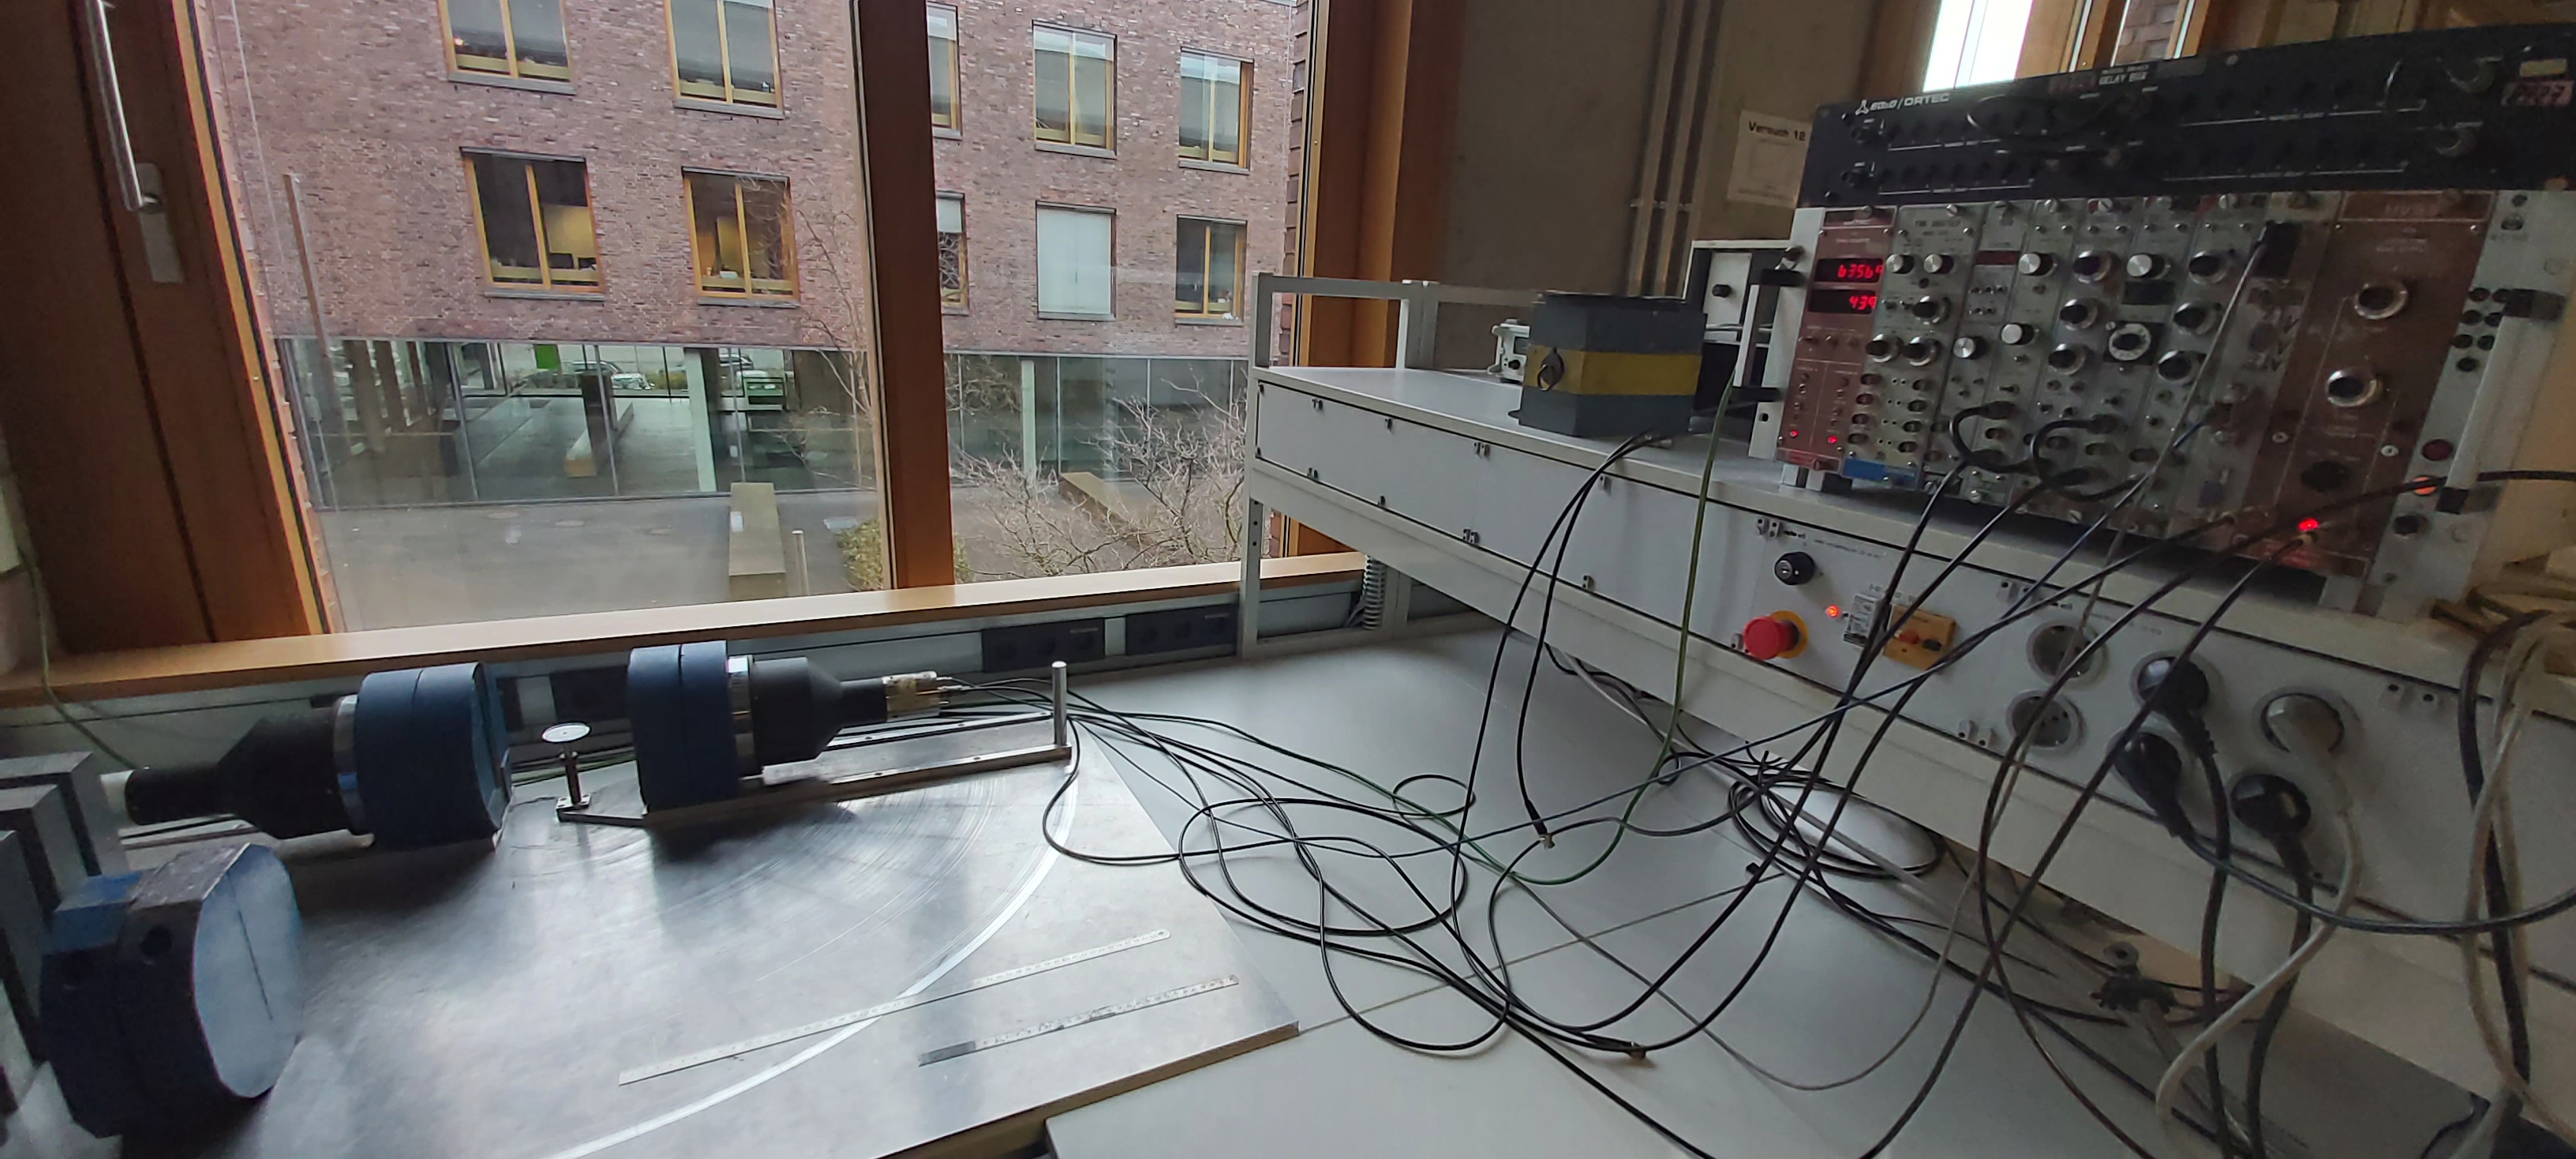
\includegraphics[scale=0.14]{images/setting.jpg}
	\caption{Versuchsaufbau. Zu erkennen sind die zwei Detektoren und die signalverarbeitende Apparatur}
	\label{fig:setting}
\end{figure}
In \ref{fig:setting} ist zu sehen, wie die Szintillationsdetektoren mit dem signalverarbeitendem Gerät verbunden sind. Die Apparatur besteht aus
\begin{itemize}
	\item dem PMT, hier als \textit{DDL Amp} bezeichnet
	\item dem \textit{Timing Single Channel Analyser} (TSCA), das das vom PMt angekommene Signal in ein starkes positives Rechtecksignal von 5V und ein schwaches negatives Rechtecksignal von -0.5V umwandelt
	\item dem \textit{Time to Pulse Height Converter} (TPHC)
	\item dem \textit{Analog to Digital Converter} (ADC), dessen \textit{Gate} die Funktion eines input gates spielt, d.h. ein einkommendes Signal anzunehmen oder zu verweigern,
	\item und dem \textit{Multi Channel Analyser}, der die Signalstärken bei den verschiedenen Kanälen darstellt.
\end{itemize}
%%%%%%%%%%%%%%%%%%%%%%%%%%%%%%%%%%%%%%%%%%%
%%%%%%%%%%%%%%%%%%%%%%%%%%%%%%%%%%%%%%%%%%%
\newpage
\section{Durchführung}
\label{sec:Durchführung und Resultate}
\subsection{Energiegesamtspektra; Kalibration Kanallage-Energie}
Um die Kanallagen als Energiewerte in keV zu interpretieren, muss eine zugehörige Kalibration durchgeführt werden. Wir beruhen uns auf die Tatsache, dass die Kanallagen des TSCA linear proportional zur Energie von einer Genauigkeit von 1keV sind (\textcolor{red}{ref old manual}):
\begin{align}
	E_{\gamma} &= a + b\cdot K,
	\label{eq:calibrate}
\end{align}
mit den zu bestimmenden Parameter $a,b$ und der Kanallage $K$. \\
Wenn in einem Spektrum zwei Werte auf bestimmten Kanallagen sitzen und deren Energiewerte bekannt sind (wie z.B. die gaußschen Peaks der Gammaquantenenergien), kann man die Parameter $a$ und $b$ bestimmen:
\begin{align}
	\Delta E_{\gamma} &= b \Delta K , \\
	b &= \frac{\Delta E_{\gamma}}{\Delta K},
\end{align}
Die Peaks der Gammaquantenenergien können neben dem visuellen Ablesen durch numerische Fits genauer bestimmt werden. Für die multimodale Verteilung der Gesamtenergiespektren verwenden wir die Pythonumgebung \texttt{emcee} (\textcolor{red}{ref emcee}), die den numerischen Fit mittels Markv-Chain-Monte-Carlo Sampling durchführt. Der Algorithmus ist dabei der Metropolis-Alorithmus und beruht sich auf den Bayesschen Satz. Die vertikalen Linien in \ref{fig:so1initial} sind zunächst visuell abgelesene Schätzungen, die für das Angeben der Priors hilfreich sind.\\
Zur Veranschaulichung werden die Plots von einem Beispiel (Natrium Detektor 1) dargestellt. Die restlichen Plots sind im Anhang zu finden.
\begin{figure}[H]
		\centering
		\includegraphics[scale=.8]{"plots/Energiegesamtspektrum von Natrium aus Detektor 1".pdf}
		\caption{Gesamtenergiespektrum von Natrium, Detektor 1.
		Die zwei Peaks sind zunächst abgeschätzt.}
		\label{fig:so1initial}
\end{figure}
Für den numerischen Fit mittels \texttt{emcee} müssen wir einen Prior angeben; eine Modellfunktion, an der sich der numerische Fit zu richten hat. Wir konstruieren die Modellfunktion als Summe dreier Verteilungsfunktionen: eine Funkiton für die Hintergrundstrahlung (lognormal bzw. exponentielle Verteilung) und zwei Normalverteilungsfunktionen für die Peaks der Gammaquantenenergien:
\begin{align}
	M(\vec{\theta}, x) &= a_1 \cdot P_{ln}((\mu_1,\sigma_1),x) + a_2 \cdot P_{N}((\mu_2,\sigma_2), x) + a_3 \cdot P_{N}((\mu_3,\sigma_3), x) \\
	P_{ln}((\mu,\sigma), x) &= \frac{1}{x \cdot \sigma \sqrt{2\pi}} \exp \left[ -\frac{1}{2} \left ( \frac{\ln x - \mu}{\sigma} \right )^2  \right] \\
    P_{gauss}((\mu,sigma), x) &= \frac{1}{\sigma \sqrt{2\pi}} \exp \left[ -\frac{1}{2} \left( \frac{x-\mu}{\sigma} \right)^2 \right ] \\
    \vec{\theta} &= (\mu_1, \mu_2, \mu_3, \sigma_1, \sigma_2, \sigma_3, a_1, a_2, a_3)^T
\end{align}
mit dem Hyperparametervektor $\vec\theta$, dessen Werte der numerische Fit bestimmt. Die Werte des Hyperparameters sind im Anhang bei den Cornerplots zu entnehmen. 
\begin{figure}[H]
	\centering
	\includegraphics[scale=.8]{"plots/MCMC Natrium Detektor 1 Chains".pdf}
	\caption{MCMC Durchlauf Natrium, Detektor 1. Rot dargestellt sind die Markov-Ketten: Modellfunktionen mit variierendem Hyperparameter.}
\end{figure}

\begin{figure}[H]
	\centering
	\includegraphics[scale=.8]{"plots/MCMC Natrium Detektor 1 Fit".pdf}
	\caption{MCMC highest likelihood Natrium, Detektor 1. Das Modell mit der höchsten Likelihood. Grau markiert ist der 1$\sigma$-Bereich.}
\end{figure}

Für die Unsicherheit der gaußschen Mittelwerte verwenden wir entsprechend die gaußschen Standardabweichungen:
\begin{table}[H]
    \centering
    \begin{tabular}{lllll}
    \hline
        		  & K$_1$ & $\sigma_1$ & K$_2$ & $\sigma_2$ \\ \hline
        Natrium D1 & 483.965 & 15.8 & 1259.43 & 51.25 \\ \hline
        Natrium D2 & 201.54 & 28.91 & 703.413883 & 48.78 \\ \hline
        Cobalt D1 & 1143.162596 & 39.92 & 1301.708396 & 34.81 \\ \hline
        Cobalt D2 & 703.413883 & 50.97 & 829.951054 & 46.65 \\ \hline
    \end{tabular}
	\caption{Erwartungswerte und Ungenauigkeiten der gaußschen Fits, entnommen von den Hyperparameters der MCMC-Fits.}
	\label{tab:mcmcerror}
\end{table}

Die Kalibrationsparameter $a$ und $b$ haben eine Unsicherheit, die durch die gaußsche Fehlerfortpflanzung bestimmt werden können: 
\begin{align}
    b                &= \frac{\Delta E_\gamma}{\Delta K} \\
    \Delta b         &=  \sqrt{ \left ( \frac{\partial b}{\partial (\Delta K)}\Delta(\Delta K) \right )^2 } \\
                     &= \frac{\Delta E_{\gamma}}{(\Delta K)^2}\Delta (\Delta K) \\
    \Delta(\Delta K) &= \sqrt{ \left( \frac{\partial(\Delta K)}{\partial K_1} \sigma_1 \right)^2 + 
        \left( \frac{\partial(\Delta K)}{\partial K_2} \sigma_2 \right)^2} \\
                     &= \sqrt{\sigma_1^2 + \sigma_2^2}\\
    a                &= E_{\gamma} - b \cdot K \\
    \Delta a         &= \sqrt{ \left( \frac{\partial a}{\partial b} \Delta b \right)^2 + 
        \left( \frac{\partial a}{\partial K} \sigma \right)^2  } \\
                     &= \sqrt{ \left( K \cdot \Delta b \right)^2 + \left( b \cdot \sigma \right)^2 }
\end{align}
Die Fehlerberechnung von $a$ entspricht dem formellen Prozess der gaußschen Fehlerfortpflanzung, weist jedoch hohe Werte auf, da sie - vor allem bei Cobalt - mit hohen Kanallagewerten $K$ skaliert, siehe dazu die Fehlerwerte in Tabelle \ref{tab:calibration}. Um qualitativ die Genauigkeit des Parameters $a$ zu untersuchen, führen wir eine weitere Kalibration mit Cobalt durch, siehe Abbildung \ref{fig:calibratecurve}. Wir erkennen dabei, dass Detektor 1 bei beiden Quellen eine beinahe gleiche Kalibration entsteht, während wir bei Detektor 2 aufgrund seiner mangelhaften Funktion eine bereits erwartete Diskrepanz sehen. Dieser visuelle Vergleich schließt die hohe Ungenauigkeit von $a$ nicht aus, regt jedoch dazu an, andere Alternativen zur gaußschen Fehlerfortpflanzung in Erwägung zu ziehen, denn der visuelle Abgleich bei Detektor 1 deutet darauf hin, dass der Parameter $a$ zu hoher Wahrscheinlichkeit den richtigen Wert annimmt.
%\begin{table}[H]
%	\centering
%	\begin{tabular}{llrr}
%	\toprule
%	&  & na & co \\
%	Theoretical / Detector & Peak &  &  \\
%	\midrule
%	\multirow[t]{2}{*}{E} & p1 & 511.0000 & 1173.2000 \\
%						  & p2 & 1275.0000 & 1332.5000 \vspace{10pt} \\
%	\cline{1-4}
%	\multirow[t]{2}{*}{D1} & p1 & 482.2678$^{+1}_{-1.64}$ & 1144.3418$^{+8.02}_{-0.63}$ \vspace{10pt}\\
%						   & p2 & 1256.6943$^{+10.46}_{-4.9}$ & 1304.5335$^{+0.87}_{-1.08}$ \vspace{10pt}\\
%	\cline{1-4}
%	\multirow[t]{2}{*}{D2} & p1 & 201.4313$^{+2.2}_{-0.34}$ & 702.5079$^{+0.29}_{-5.47}$ \vspace{10pt}\\
%						   & p2 & 784.0605$^{+3.5}_{-2.76}$ & 829.7451$^{+0.58}_{-13.17}$ \\
%	\cline{1-4}
%	\bottomrule
%	\end{tabular}
%	\caption{Peaks im Spektrum. Werte sind von den Cornerplots der Hyperparametervektoren zu entnehmen.}
%	\label{tab:peaks}
%\end{table}

\begin{table}[H]
	\centering
	\begin{tabular}{llrrrr}
	\toprule
	 &  & Natrium & Fehlerwert & Cobalt & Fehlerwert \\
	Detektor & Kalibrationsparameter &  &  &  &  \\
	\midrule
	\multirow[t]{2}{*}{D1} & a & 34.1903 & 36.4651 & 24.5994 & 385.8043 \\
	 & b & 0.9852 & 0.0681 & 1.0048 & 0.3357 \\
	\cline{1-6}
	\multirow[t]{2}{*}{D2} & a & 204.1967 & 50.6115 & 287.6592 & 487.7864 \\
	 & b & 1.5223 & 0.1240 & 1.2589 & 0.6874 \\
	\cline{1-6}
	\bottomrule
	\end{tabular}
\caption{Parameter der Kalibration}
\label{tab:calibration}
\end{table}

%\begin{table}[H]
%	\centering
%	\begin{tabular}{llrr}
%	\toprule
%	&  & Na & Co \\
%	Detektor & Kalibrationsparameter &  &  \\
%	\midrule
%	\multirow[t]{2}{*}{D1} & a & 35.2252 & 35.2281 \\
%	 & b & 0.9865 & 0.9944 \\
%	\cline{1-4}
%	\multirow[t]{2}{*}{D2} & a & 246.8638 & 293.6654 \\
%	 & b & 1.3113 & 1.2520 \\
%	\cline{1-4}
%	\bottomrule
%	\end{tabular}
%
%\end{table}

\begin{figure}[H]
	\centering
	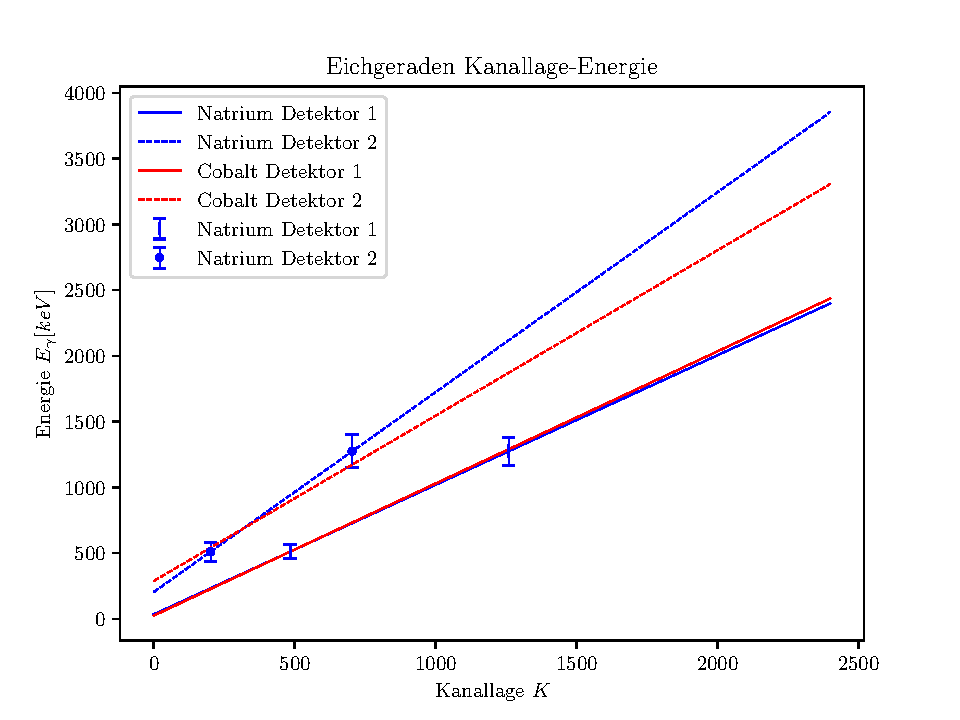
\includegraphics[scale=.9]{plots/Eichgeraden.pdf}
	\caption{Eichgerade. Es wurde sowohl eine Natrium, als auch eine Cobalt Eichung durchgeführt. Zweck ist der qualitative Vergleich der Detektoren und der Kalibrationsungenauigkeit.}
	\label{fig:calibratecurve}
\end{figure}
Wir verwenden nun die Natriumeichung, um die die Energie für eine gegebene Kanallage gemäß \ref{eq:calibrate} zu bestimmen. Ein kalibriertes Gesamtspektrum ist in Abbildung \ref{fig:calibratespectrum} zu sehen, für den Rest siehe Anhang \ref{fig:calibratedsodium1} bis \ref{fig:calibratedcobalt2}. Gemäß der Fehlerrechnung ergibt sich bei beiden Detektoren jeweils ein Energiewert von
\begin{align}
	E_{\gamma, D1} (\text{in $keV$})&= (0.9852 \pm 0.0681)\cdot K + (34.1903 \pm 36.4651)\\
	E_{\gamma, D2} (\text{in $keV$})&= (1.5223 \pm 0.1240)\cdot K + (204.1967 \pm 50.6115) 
\end{align}
\begin{figure}[H]
	\centering
	\includegraphics[scale=.9]{"plots/Kalibriertes Energiegesamtspektrum von Cobalt aus Detektor 1".pdf}
	\caption{Kalibriertes Energiegesamtspektrum von Cobalt aus Detektor 1. Bei allen vier Plots wird die Natriumeichung verwendet.}
	\label{fig:calibratespectrum}
\end{figure}
\subsection{Time-delay Spektra, Kalibration Kanallage-Zeit}
Wir führen eine zum vorherigen Abschnitt analoge Kalibration durch. In diesem Fall haben wir es mit einer unimodalen Verteilung zu tun, weshalb wir für den numerischen Fit die Umgebung \texttt{scipy.optimize} verwenden. Der Vorteil hierbei ist, dass der Fit deutlich schneller fertig ist. Als Vergleich wird noch eine "per Hand" berechnete, analytische Gaußfunktion zum Verleich dargestellt. Die parametrisierten Fits sind in den Abbildungen \ref{fig:timedelay} zu sehen. 
\begin{figure}[H]
	\centering
	\includegraphics[scale=.8]{"plots/Vergleich gaußscher Fits bei 0ns Delay".pdf}
	\caption{numerischer Fit für 0ns}
	\label{fig:timedelay}
\end{figure}
\begin{figure}[H]
	\centering
	\includegraphics[scale=.8]{"plots/Vergleich gaußscher Fits bei 96ns Delay".pdf}
	\caption{numerischer Fit für 96ns}
\end{figure}
Zum Abgleich der Kalibration verwenden wir hier die Zeitdifferenz von 96ns und 0ns und die Differenz in den Peaks der Kanallagen:
\begin{align}
	\Delta t &= 96ns = b \cdot \Delta K. 
\end{align}
Für die Fehlerfortpflanzung verwenden wir die vom numerischen Fit gegebenen Standardabweichungen $\sigma_{0}=$100.3792 und $sigma_{96}= 100.74068$:
\begin{align}
    \Delta b &= \frac{\Delta t}{(\Delta K)^2} \Delta(\Delta K) \\
    \Delta (\Delta K) &= \sqrt{ \sigma_1^2 + \sigma_2^2 }.
\end{align}
Die Eichgerade ist in Abbildung \ref{fig:timecalibrate} zu sehen. Wir kommen auf eine Kalibration von
\begin{align}
	t (\text{in $ns$})&= (0.14269008508992875 \pm 0.030161790372228194) \cdot K \\
	\Delta t_{i} &= \sqrt{ (K_i \Delta b)^2 + (b \sigma_i)^2 }
\end{align}
mit $i $= 0$ns$, 96$ns$.
\begin{figure}[H]
	\centering
	\includegraphics[scale=.8]{"plots/Eichgerade Zeit".pdf}
	\caption{Eichgerade Kanallage-Zeit}
	\label{fig:timecalibrate}
\end{figure}
		Mit der Zeiteichung können wir die Zeitauflösung bestimmen. Sie ergibt sich aus der Bestimmung der Breite der Gaußen Verteilungen bei halber Höhe (FWHM: Full Width at Half Maximum). Der x-Wert bei halber Höhe wird numerisch mit \texttt{numpy.interp} bestimmt, in dessen Dokumentation keine Ungenauigkeitbestimmung gegeben ist. Die Ungenauigkeit bestimmen wir daher nur im Bezug auf die Ungenauigket des Kalibrationsparameters:
\begin{align}
	\Delta \text{FWHM} &= \sqrt{ (x_2 - x_1)^2\Delta^2 b }.
\end{align}
Als Endwerte bekommen wir
\begin{table}[H]
	\centering
	\begin{tabular}{lll}
		\toprule
			Zeitdelay & FWHM         & Fehler \\
		\midrule
			0$ns$     & 32.80362$ns$ & 6.93402$ns$ \\
		\cline{1-3}
			96$ns$    & 32.96602$ns$ & 6.96835$ns$ \\
		\cline{1-3}
		\bottomrule
	\end{tabular}
	\caption{FWHM Werte mit Ungenauigkeiten}
	\label{tab:fwhm}
\end{table}

\newpage
\subsection{Koinzidenzmessungen}
\noindent \textbf{$e^+e^-$ Annihilation (511keV - 511keV)}\\
	Es wird die Vernichtungsstrahlung von den Positronen aus der Natriumquelle bei verschiedenen kleinen Winkelauslenkungen betrachtet:

\begin{table}[H]
    \centering
    \begin{tabular}{llll}
    \hline
        Auslenkung & Gesamtzahl $Z$ & Gesamtmesszeit $T$ & Zählraten $Q$\\ \hline
        0cm & 24 & 123.136s & 0.1949064449064449 $s^{-1}$ \\ \hline
        -1cm & 59 & 123.155s & 0.47907108927773945 $s^{-1}$ \\ \hline
        -2cm & 84 & 129.882s & 0.6467408878828474 $s^{-1}$ \\ \hline
        -3cm & 48 & 122.609s & 0.3914883899224364 $s^{-1}$ \\ \hline
    \end{tabular}
	\caption{Zählraten bei verschiedenen Auslenkungen für die Vernichtungsstrahlung}
	\label{tab:coincidenceannihilation}
\end{table}

Eine grafische Darstellung ist in \ref{fig:coincidenceannihilation} zu sehen. Für die Ungenauigkeit in der Auslenkung werden 0.2$cm$ angenommen, während die Ungenauigkeit der Gesamtzahl sich in die Ungenauigkeit der Zählrate fortpflanzt. Die Gesamtzahl ist eine diskrete, poissonverteilte Größe, deren Standardabweichung die Wurzel des Erwartungswertes ist. So gilt dann für die Ungenauigkeit der Zählrate $Q$:
\begin{align}
	\Delta Q &= \sqrt{ \left( \frac{1}{T}\sqrt{Z}  \right)^2  }
\end{align}

\begin{figure}[H]
	\centering
	\includegraphics[scale=0.8]{"plots/Koinzidenzplot Vernichtungsstrahlung".pdf}
	\caption{grafische Darstellung der $\gamma - \gamma -$Koinzidenz für die Vernichtungsstrahlung}
	\label{fig:coincidenceannihilation}
\end{figure}

\textbf{$e^+e^- $ Annihilation und $\gamma$-Zerfall (511keV - 1275keV)}\\
Es wird erwartet, dass die gemessenen Zählraten kleiner werden als beim vorherigen Versuch. Dies konnte in unserem Fall nicht bestätigt werden. Eine grafische Darstellung ist in Abbildung \ref{fig:coincidenceannihilgamma} zu sehen. Wir erwarten aus der Theorie keine Koinzidenz zwischen den Gammaquanten der Vernichtung und des Gammazerfalls, da die zwei Prozesse unabhängig voneinander ablaufen. Wir erwarten also keine Zeitgleichheit aus einem kausalen Zusammenhang. Aufgrund unserer endlichen Auflösung ist jedoch zu erwarten, dass das Zeitfenster zwischen erstem und zweiten Gammaquant sehr kurz ist, und zu zufälligen Koinzidenzen führen kann. \\
Würde eine Koinzidenz existieren, müssen wir in der Abblidung eine Winkelabhängigkeit gemäß der Winkelkorrelationsfunktion erkennen.

\begin{figure}[H]
	\centering
	\includegraphics[scale=0.8]{"plots/Koinzidenzplot Vernichtungsstrahlung Gammazerfall".pdf}
	\caption{grafische Darstellung der $\gamma - \gamma -$Koinzidenzmessung für die Vernichtungsstrahlung und den Gammazerfall}
	\label{fig:coincidenceannihilgamma}
\end{figure}

\textbf{Koinzidenzmessung Cobalt}
\textcolor{red}{table coincidence analytics}

\begin{figure}[H]
	\centering
	\includegraphics[scale=0.8]{"plots/Winkelkorrelationen Vergleich".pdf}
	\caption{Vergleich der Winkelkorrelationsfunktion von gemessenen Daten und von der Theorie}
	\label{fig:coincidencecobalt}
\end{figure}

%%%%%%%%%%%%%%%%%%%%%%%%%%%%%%%%%%%%%%%%%%%
%%%%%%%%%%%%%%%%%%%%%%%%%%%%%%%%%%%%%%%%%%%



\section{Diskussion}
\label{sec:Diskussion}
\textbf{Zu den kalibrierten Spektren von Cobalt}\\
Wie wir im Anhang bei der Platzierung der theoretischen Peaks erkennen können, ist die Kalibration nur beim Detektor 1 gelungen, während die Kalibration für den Detektor 2  


%%%%%%%%%%%%%%%%%%%%%%%%%%%%%%%%%%%%%%%%%%%
%%%%%%%%%%%%%%%%%%%%%%%%%%%%%%%%%%%%%%%%%%%




\section{Fazit}
\label{sec:Fazit}



%%%%%%%%%%%%%%%%%%%%%%%%%%%%%%%%%%%%%%%%%%%
%%%%%%%%%%%%%%%%%%%%%%%%%%%%%%%%%%%%%%%%%%%
\interlinepenalty=10000
\section{Quellen}
\bibliography{report.bib}

%%%%%%%%%%%%%%%%%%%%%%%%%%%%%%%%%%%%%%%%%%%
%%%%%%%%%%%%%%%%%%%%%%%%%%%%%%%%%%%%%%%%%%%


\section{Anhang}
\label{sec:Anhang}
\begin{figure}[ht]
	\label{fig:initialplotsSo}
	\begin{subfigure}[c]{0.8\textwidth}
		\includegraphics[width=\textwidth]{"plots/Energiegesamtspektrum von Natrium aus Detektor 1".pdf}
		\subcaption{Natrium, Detektor 1}
	\end{subfigure}

	\begin{subfigure}[c]{0.8\textwidth}
		\includegraphics[width=\textwidth]{"plots/Energiegesamtspektrum von Natrium aus Detektor 2".pdf}
		\subcaption{Natrium, Detektor 2}
	\end{subfigure}
\end{figure}

\begin{figure}[ht]
	\label{fig:initialplotsCo}
	\begin{subfigure}[c]{0.8\textwidth}
		\includegraphics[width=\textwidth]{"plots/Energiegesamtspektrum von Cobalt aus Detektor 1".pdf}
		\subcaption{Cobalt, Detektor 1}
	\end{subfigure}

	\begin{subfigure}[c]{0.8\textwidth}
		\includegraphics[width=\textwidth]{"plots/Energiegesamtspektrum von Cobalt aus Detektor 2".pdf}
		\subcaption{Cobalt, Detektor 2}
	\end{subfigure}

\end{figure}
\begin{figure}		
	\includegraphics[scale=.3]{"plots/MCMC Natrium Detektor 1 Hyperparameters".pdf}
	\caption{MCMC Hyperparameter corner plot, Natrium, Detektor 1.}
\end{figure}

\begin{figure}		
	\includegraphics[scale=.8]{"plots/Kalibriertes Energiegesamtspektrum von Natrium aus Detektor 1".pdf}
	\caption{kalibriertes Spektrum Natrium, Detektor 1.}
	\label{fig:calibratedsodium1}
\end{figure}
\begin{figure}		
	\includegraphics[scale=.8]{"plots/Kalibriertes Energiegesamtspektrum von Natrium aus Detektor 2".pdf}
	\caption{kalibriertes Spektrum Natrium, Detektor 2.}
\end{figure}
\begin{figure}		
	\includegraphics[scale=.8]{"plots/Kalibriertes Energiegesamtspektrum von Cobalt aus Detektor 2".pdf}
	\caption{kalibriertes Spektrum Cobalt, Detektor 2.}
	\label{fig:calibratedcobalt2}
\end{figure}

\end{document}
